Nous nous intéressons à présent à la complexité de l'algorithme générique (algorithme
\ref{algo_generic} p. \pageref{algo_generic}). Afin de pouvoir calculer cette dernière, nous allons
avoir besoin de quelques bornes utiles.

\begin{lemma} ~\\
	\label{increase_distance}
	Chaque opération de réétiquetage d'un noeud augmente strictement sa distance $d$ au noeud puits.
\end{lemma}

\textbf{Preuve} \\
Considérons un noeud actif $i$ soumis à une opération de poussage-réétiquetage. Supposons, à présent,
qu'il existe un noeud $j$ tel que après réétiquetage on ait : $d_{new}(i) \leq d_{old}(i)$. Ceci
n'est possible que si $d(j) \leq d(i) - 1$ et si $r_{ij}$\footnote{La capacité résiduelle de l'arc
$(i,j)$}$\geq 0$, on aurait alors $(i,j) \in A_i$ ce qui signifie alors que l'algorithme aurait
effectué une opération de poussage et non un réétiquetage. Il est donc impossible de trouver un
noeud $j$ tel que l'opération de réétiquetage diminue sa distance $d$.

\begin{lemma} ~\\
	\label{residual_path}
	A n'importe quelle itération de l'algorithme, tout noeud actif $i$ est relié au noeud source $s$ par un
	chemin de $i$ vers $s$ dans le réseau résiduel.
\end{lemma}

\textbf{Preuve}\\
D'après le théorème de décomposition des flots\footnote{Un exemple d'application de ce théorème est
donné à la figure \ref{app_dec_preflot}}, il est possible de décomposer n'importe quel préflot
en des flots positifs le long de chemins reliant $s$ à $t$ \footnote{Le noeud puits}, $s$ aux noeuds
actifs et le long de cycles. De plus par définition d'un préflot on a : $e(s) \leq 0$ et $e(i) \geq
0 \ \forall i \in S - \{s\}$.

\begin{figure}
	\begin{center}
		\subfloat[Un préflot]{
		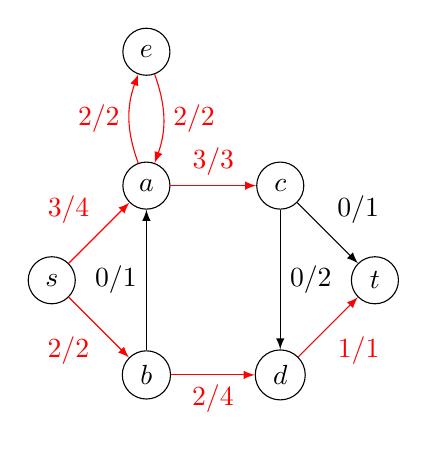
\begin{tikzpicture}[node distance=1.7cm]
			\tikzset{n/.style={draw=black, circle, minimum width=17pt},
			f/.style={->, >=latex}};

			\node[n] (s) at (0,0) {$s$};
			\node[n, above right of=s] (a) {$a$};
			\node[n, below right of=s] (b) {$b$};
			\node[n, above of=a] (e) {$e$};
			\node[n, right of=a] (c) {$c$};
			\node[n, right of=b] (d) {$d$};
			\node[n, above right of=d] (t) {$t$};

			\draw[f, red] (s) to node[above left, red] {$3/4$} (a);
			\draw[f, red] (s) to node[below left, red] {$2/2$} (b);
			\draw[f, red] (a) to[out=110, in=250] node[left, red] {$2/2$} (e);
			\draw[f, red] (e) to[out=290, in=70] node[right, red] {$2/2$} (a);
			\draw[f, red] (a) to node[above, red] {$3/3$} (c);
			\draw[f, red] (b) to node[below, red] {$2/4$} (d);
			\draw[f, red] (d) to node[below right, red] {$1/1$} (t);
			\draw[f] (c) to node[above right] {$0/1$} (t);
			\draw[f] (b) to node[left] {$0/1$} (a);
			\draw[f] (c) to node[right] {$0/2$} (d);
	\end{tikzpicture}}\hfill
	\subfloat[La décomposition en flots de $s$ vers $t$]{
		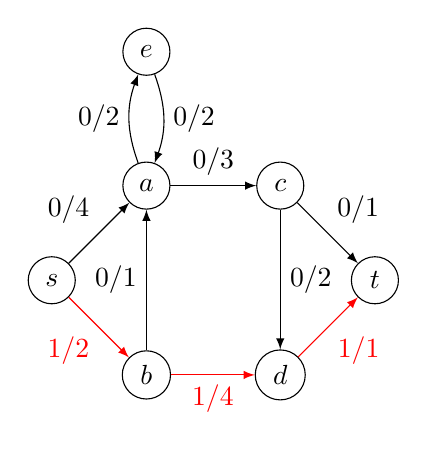
\begin{tikzpicture}[node distance=1.7cm]
			\tikzset{n/.style={draw=black, circle, minimum width=17pt},
			f/.style={->, >=latex}};

			\node[n] (s) at (0,0) {$s$};
			\node[n, above right of=s] (a) {$a$};
			\node[n, below right of=s] (b) {$b$};
			\node[n, above of=a] (e) {$e$};
			\node[n, right of=a] (c) {$c$};
			\node[n, right of=b] (d) {$d$};
			\node[n, above right of=d] (t) {$t$};

			\draw[f] (s) to node[above left] {$0/4$} (a);
			\draw[f, red] (s) to node[below left, red] {$1/2$} (b);
			\draw[f] (a) to[out=110, in=250] node[left] {$0/2$} (e);
			\draw[f] (e) to[out=290, in=70] node[right] {$0/2$} (a);
			\draw[f] (a) to node[above] {$0/3$} (c);
			\draw[f, red] (b) to node[below, red] {$1/4$} (d);
			\draw[f, red] (d) to node[below right, red] {$1/1$} (t);
			\draw[f] (c) to node[above right] {$0/1$} (t);
			\draw[f] (b) to node[left] {$0/1$} (a);
			\draw[f] (c) to node[right] {$0/2$} (d);
		\end{tikzpicture}}\hfill
	\subfloat[La décomposition en flots de $s$ vers les n\oe uds actifs]{
		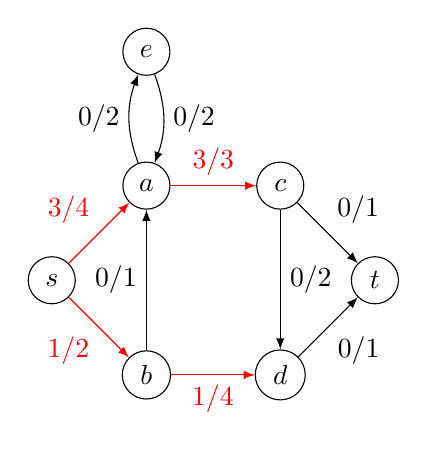
\begin{tikzpicture}[node distance=1.7cm]
			\tikzset{n/.style={draw=black, circle, minimum width=17pt},
			f/.style={->, >=latex}};

			\node[n] (s) at (0,0) {$s$};
			\node[n, above right of=s] (a) {$a$};
			\node[n, below right of=s] (b) {$b$};
			\node[n, above of=a] (e) {$e$};
			\node[n, right of=a] (c) {$c$};
			\node[n, right of=b] (d) {$d$};
			\node[n, above right of=d] (t) {$t$};

			\draw[f, red] (s) to node[above left, red] {$3/4$} (a);
			\draw[f, red] (s) to node[below left, red] {$1/2$} (b);
			\draw[f] (a) to[out=110, in=250] node[left] {$0/2$} (e);
			\draw[f] (e) to[out=290, in=70] node[right] {$0/2$} (a);
			\draw[f, red] (a) to node[above, red] {$3/3$} (c);
			\draw[f, red] (b) to node[below, red] {$1/4$} (d);
			\draw[f] (d) to node[below right] {$0/1$} (t);
			\draw[f] (c) to node[above right] {$0/1$} (t);
			\draw[f] (b) to node[left] {$0/1$} (a);
			\draw[f] (c) to node[right] {$0/2$} (d);
		\end{tikzpicture}}\\
	\subfloat[La décomposition en cycles]{
		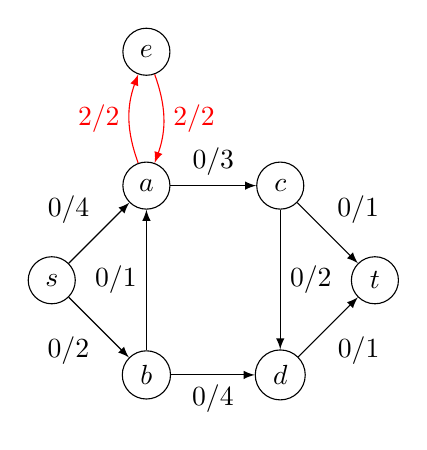
\begin{tikzpicture}[node distance=1.7cm]
			\tikzset{n/.style={draw=black, circle, minimum width=17pt},
			f/.style={->, >=latex}};

			\node[n] (s) at (0,0) {$s$};
			\node[n, above right of=s] (a) {$a$};
			\node[n, below right of=s] (b) {$b$};
			\node[n, above of=a] (e) {$e$};
			\node[n, right of=a] (c) {$c$};
			\node[n, right of=b] (d) {$d$};
			\node[n, above right of=d] (t) {$t$};

			\draw[f] (s) to node[above left] {$0/4$} (a);
			\draw[f] (s) to node[below left] {$0/2$} (b);
			\draw[f, red] (a) to[out=110, in=250] node[left, red] {$2/2$} (e);
			\draw[f, red] (e) to[out=290, in=70] node[right, red] {$2/2$} (a);
			\draw[f] (a) to node[above] {$0/3$} (c);
			\draw[f] (b) to node[below] {$0/4$} (d);
			\draw[f] (d) to node[below right] {$0/1$} (t);
			\draw[f] (c) to node[above right] {$0/1$} (t);
			\draw[f] (b) to node[left] {$0/1$} (a);
			\draw[f] (c) to node[right] {$0/2$} (d);
		\end{tikzpicture}}
	\end{center}
	\caption{Un exemple de décomposition de préflot, d'après le théorème de décomposition des flots}
	\label{app_dec_preflot}
\end{figure}

Considérons un noeud actif $i$, l'excès de flots $e(i)$ est strictement supérieur à $0$. Or, lors de la
considération des flots obtenus par le théorème de décomposition des flots, on observe que les flots
pris le long des cycles et des chemins de $s$ à $t$ n'interviennent pas dans l'excédent de flot de
$i$, ce qui implique qu'il existe un flot strictement positif coulant le long d'un chemin de $s$ à
$i$ et donc que l'inverse de ce chemin se trouve dans le réseau résiduel. D'où l'existence d'un chemin
de $i$ vers $s$ dans le réseau résiduel.\\

On peut directement déduire de ce lemme que, pour un noeud actif $i$, il existe toujours un
noeud de son voisinage $j$ tel que $d(j) > d(i)$ et donc que lors d'un réétiquetage, la
minimisation de la hauteur des voisins ne se fait pas sur un ensemble vide. Autrement dit, pour un
n\oe ud que l'on réétiquete, il existe toujours un sommet de son voisinage dont la distance au puits
est supérieure au n\oe ud réétiqueté.

\begin{lemma} ~\\
	\label{borne_reetiq}
	Pour tout $i \in S,\ d(i) < 2n$
\end{lemma}

\textbf{Preuve}\\
Une opération de réétiquetage d'un sommet $i$ n'affecte que la distance de $i$ au noeud puits, par conséquent
l'excédent de flot sur le noeud $i$ après l'opération est le même qu'avant. D'après le lemme
\ref{residual_path}, il existe donc un chemin $P$ de $s$ à $i$\footnote{$i \ne t$} dans le réseau
résiduel dont la longueur est au plus $n-2$ sommets\footnote{Le chemin ne peut inclure $t$, de plus
$i$ ne peut être un voisin direct de $t$, sinon il n'y aurait pas eu d'opération de réétiquetage.}.
À la fin de l'initialisation : $d(s) = |S| = n$, et pour chaque arc $(k,l)$ du chemin de $i$ à $s$,
on a : $d(k) \leq d(l) + 1$. Prenons un exemple concret, soit $G$ un graphe à 8 sommets de sorte
qu'après un certains nombre d'itérations de l'algorithme, le noeud $6$ est actif\footnote{Il s'agit
bien du pire des cas : une chaîne de $n-2$ sommets}. Le chemin de $6$ vers $s$ est représenté à la
fig. \ref{chemin_n_2}. 

\begin{figure}
	\begin{center}
		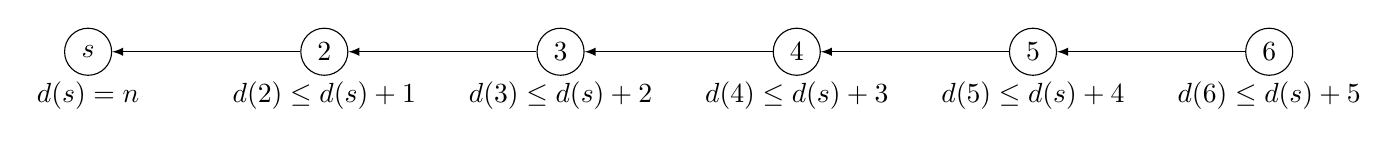
\begin{tikzpicture}[node distance=16pt]
			\tikzset{node/.style={circle, draw=black, minimum width=17pt, inner sep = 0pt}};
			\node[node] (1) at ( 0,0) {$s$};
			\node[node] (2) at ( 3,0) {$2$};
			\node[node] (3) at ( 6,0) {$3$};
			\node[node] (4) at ( 9,0) {$4$};
			\node[node] (5) at (12,0) {$5$};
			\node[node] (6) at (15,0) {$6$};

			\node (a1) [below of=1] {$d(s) = n$};
			\node (a2) [below of=2] {$d(2) \leq d(s) + 1$};
			\node (a3) [below of=3] {$d(3) \leq d(s) + 2$};
			\node (a4) [below of=4] {$d(4) \leq d(s) + 3$};
			\node (a5) [below of=5] {$d(5) \leq d(s) + 4$};
			\node (a6) [below of=6] {$d(6) \leq d(s) + 5$};


			\draw[<-, >=latex] (1) -- (2);
			\draw[<-, >=latex] (2) -- (3);
			\draw[<-, >=latex] (3) -- (4);
			\draw[<-, >=latex] (4) -- (5);
			\draw[<-, >=latex] (5) -- (6);
		\end{tikzpicture}
	\end{center}
	\caption{Chemin de longueur $n-2$ sommets dans le graphe résiduel}
	\label{chemin_n_2}
\end{figure}

En partant de $d(s) = n$, on peut écrire : $$
d(2) \leq d(s) + 1 $$ Or on a aussi : $$
\begin{array}{lrcl}
	&d(3) & \leq & d(2) + 1 \\
\Rightarrow & d(3) & \leq & d(s) + 2
\end{array} $$

Donc pour le $n-2^e$ sommet on a : $$
\begin{array}{lrcl}
	&d(n-2) &\leq& d(s) + (n - 3) \\
\Rightarrow & d(n-2) & < & d(s) + n \\
\Rightarrow & d(n-2) & < & 2n 
\end{array} $$

Et comme il s'agit du pire des cas, on peut généraliser : $\forall i \in S, \quad d(i) < 2n $.
Si l'on prend en compte le fait qu'à chaque opération de réétiquetage, la distance $d$ est augmentée
au minimum d'une unité, on obtient le lemme \ref{borne_n2}.

\begin{lemma}~\\
	\label{borne_n2}
	Un noeud $i$ subit au maximum $2n$ opération de réétiquetage, ce qui implique que le nombre total
	d'opération de réétiquetage est borné par $2n^2$
\end{lemma}

\begin{lemma}~\\
	\label{borne_ps}
	Le nombre de poussages saturants\footnote{Un poussage de $i$ vers $j$ est dit saturant si après
	poussage, $r((i,j)) = 0$} exécutés pendant l'algorithme est inférieur à $2nm$.
\end{lemma}

\textbf{Preuve}\\
Considérons deux sommets voisins $i$ et $j$. Si l'on considère un poussage saturant de $i$ vers
$j$ (respectivement de $j$ vers $i$), alors l'arête $(j, i)$ (resp. $(i,j)$) est une arête de $A_f$.
Pour pouvoir effectuer le poussage saturant inverse, $j$ (resp. $i$) doit augmenter sa distance de
: $d(j) - d(i) + 1$ (resp. $d(i) - d(j) + 1$) $\geq 2$. Donc chacun des sommets peut au maximum
effectuer $n$ poussages saturants vers l'autre\footnote{La distance de chaque sommet est bornée
ainsi : $0 \leq d(i) \leq 2n$, le nombre maximum d'augmentation de $d$ de 2 unités est donc $n$.}.
Ce qui nous donne pour chaque arc, un nombre de poussages saturants inférieur à $2n$. Sur
l'ensemble de l'algorithme ce dernier est bien majoré par $2nm$.

\begin{lemma}~\\
	\label{borne_pns}
	Le nombre de poussage non saturants lors de l'exécution de l'algorithme est borné supérieurement
	par $O(n^2m)$.
\end{lemma}

\textbf{Preuve}\\
Considérons la fonction $\Phi$ qui calcule la somme des distances des noeuds actifs : $$
\Phi = \sum_{i \in \{i \in S / e(i) > 0\}} d(i)$$. Comme le nombre de noeuds actifs est inférieur à
$|S|$ et que la distance de chaque somme est bornée par $2n$, la valeur initiale\footnote{Après
initialisation.} de $\Phi$ est inférieure à $2n^2$, à la fin de l'algorithme, il n'existe plus de
sommets actifs, et donc : $\Phi = 0$.
Lors du déroulement de l'algorithme, trois choses peuvent se produire : \begin{enumerate}
	\item Poussage non saturant. Il a lieu lorsque l'excédent de préflot du sommet est inférieur à la
		capacité résiduelle de l'arc emprunté, donc une fois cette étape effectuée le noeud $i$ ayant
		effectué le poussage n'est plus actif. Dans le cas ou $j$, le sommet cible du poussage
		n'appartenait pas à l'ensemble des n\oe uds débordants $I$, la fonction $\Phi$ est incrémentée de 
		$d(j)$ et décrémentée de $d(i)$.  Or $d(i) \geq d(j) + 1$, donc $\Phi$ diminue d'au moins une
		unité.
	\item Poussage saturant. Il a lieu lorsque $e(i) \geq r((i,j))$, Dans le pire des cas, $j \not
		\in I$ avant l'opération, on a alors une augmentation maximale de $\Phi$ égale à la hauteur max
		de $j$, soit $2n$ donc une augmentation de $2n^2m$ pour l'ensemble des poussages saturants.
	\item Ré-étiquetage. Cette opération n'a lieu que lorsqu'aucun arc sortant de $i$ n'est valide
		pour une opération de poussage, il est évident que chaque opération de réétiquetage augmente
		$\Phi$ de $2n$ unités au maximum par noeud\footnote{Limite donnée par la hauteur maximale d'un
		noeud.}, soit une augmentation totale de $n^2$ unités sur l'ensemble de l'algorithme.
\end{enumerate}

La seule opération permettant de diminuer la valeur de $\Phi$ est un poussage non saturant, or la
valeur finale de $\Phi$ est zéro, on en déduit donc que la valeur maximale de $\Phi$ nous donne le
nombre de poussages non saturants. La valeur maximal de $\Phi$ nous est donnée par la somme des
bornes de la valeur initiale et des augmentations dues aux opérations de poussages saturants et de
réétiquetage soit : $$
\Phi = n^2 + n^2 + 2n^2m = 2n^2 (m + 1) = O(n^2m) $$

On en déduit donc le théorème suivant :
\begin{thrm}
	L'algorithme de préflots générique s'exécute en un temps $O(n^2m)$.
\end{thrm}


